\chapter{Diseño e implementación} % Main chapter title

\label{Chapter3}

En este capítulo se describe la arquitectura global del prototipo, se detalla cada módulo hardware y software que lo compone, y se documentan las decisiones de implementación, los criterios de diseño y las pruebas preliminares realizadas. Se explican los flujos de datos entre el dispositivo de campo, el broker MQTT, el backend (API REST) y la interfaz web, y se resumen las consideraciones para el despliegue y el monitoreo post-implantación.


\section{Arquitectura del sistema}

La arquitectura propuesta separa de forma explícita el dispositivo de campo (contador + ESP32-C3 + SIM800L), el transporte de mensajes (broker MQTT) y los servicios de aplicación (API REST, persistencia y frontend). Esta separación facilita la interoperabilidad y permite desplegar la solución de forma local, remota o híbrida según las políticas institucionales


\subsection{Flujo de datos} 

\begin{itemize}

  \item Detección: el contador detecta un paso y envía una trama por RS-232 al ESP32-C3.

  \item Preprocesado en nodo: el firmware valida la trama, añade sello temporal y metadatos, y encola el evento en memoria (FIFO).

  \item Transmisión: cuando la conexión GPRS está disponible, el nodo publica el evento en el tópico MQTT \texttt{devices/\{device\_id\}/events}.
  
  \item Ingesta y persistencia: el broker Mosquitto entrega el mensaje al suscriptor backend, el servicio valida el payload y persiste el registro en la base de datos MySQL.
  
  \item Visualización/Control: la interfaz web consulta la API REST para datos históricos y recibe notificaciones en tiempo real.
  
  \item Emisión de comandos (desde UI): el operador genera un comando en la interfaz, la UI envía \texttt{POST /api/devices/\{id\}/commands} al backend, que crea un \texttt{cmd\_id} único y publica en \texttt{devices/\{device\_id\}/commands}.
  
  \item Recepción en nodo y entrega al contador: el ESP32-C3, suscrito a \texttt{devices/\{device\_id\}/commands}, recibe el comando, valida \texttt{cmd\_id} y lo envía al contador por RS-232, se aplica un timeout configurable por comando.
  
  \item Ejecución y ack: el contador ejecuta la orden y responde por RS-232, el firmware publica el ack/resultado en \texttt{devices/\{device\_id\}/status} con \texttt{cmd\_id} y \texttt{status} (\texttt{ok}, \texttt{failed}, \texttt{timeout}).

  \item Actualización en backend y UI: el suscriptor MQTT del backend recibe el ack, actualiza la tabla \texttt{commands} (campo \texttt{status}, \texttt{ack\_ts}) y notifica a la UI para que el operador vea el resultado.
\end{itemize}


\subsection{Descripción ampliada de bloques y responsabilidades}
\begin{itemize}

  \item {Bloque  Dispositivo de campo.}
El nodo de campo integra el contador existente (salida RS-232), un microcontrolador ESP32-C3 y un módem GPRS SIM800L. El firmware, desarrollado sobre \texttt{ESP-IDF}, realiza las siguientes funciones: lectura continua de la trama serial, parsing tolerante a ruido, preprocesado (validación, normalización de campos y asignación de sello temporal UTC), encolamiento FIFO de eventos, gestión de reintentos y publicación MQTT cuando hay conectividad. Además, el nodo se suscribe a los tópicos de comandos y publica telemetría y acks. En el nodo se implementa persistencia mínima (registro de comandos pendientes y últimas N tramas) para recuperación tras reinicio.

  \item {Bloque Transporte (broker MQTT).}
El broker actúa como bus de mensajes desacoplado. Se recomienda emplear \textit{Eclipse Mosquitto} en la etapa inicial y evaluar brokers gestionados para despliegues a mayor escala. El broker gestiona autenticación por credenciales, control de tópicos y, en producción, cifrado TLS. Se emplean tópicos jerárquicos por dispositivo para facilitar filtrado y autorización: 
\begin{itemize}
  \item \texttt{devices/\{device\_id\}/events}
  \item \texttt{devices/\{device\_id\}/commands} 
   \item \texttt{devices/\{device\_id\}/status}.
\end{itemize}


  \item {Bloque Servidor central.}
El servidor central reúne dos responsabilidades principales: (a) componente suscriptor MQTT que valida, transforma y enruta mensajes hacia la lógica de negocio y la persistencia; y (b) API REST que expone servicios de consulta, gestión y emisión de comandos. Esta separación permite que consumidores adicionales (por ejemplo, módulos analíticos) se suscriban al broker sin impactar la disponibilidad de la API. La persistencia se implementa en MySQL con un esquema relacional que soporta consultas por rango temporal, índices para rendimiento y auditoría de comandos.

  \item {Bloque Cliente / visualización.}
La interfaz web consume la API REST para consultas históricas y utiliza WebSocket o SSE para recibir eventos en tiempo real. Se eligió Ionic + Angular por su compatibilidad con entornos de escritorio y móviles y por facilitar un despliegue unificado. Las funciones principales del cliente son: visualización de eventos en tiempo real, consulta histórica filtrada, envío de comandos remotos con seguimiento de estado y panel de telemetría para mantenimiento preventivo.
\end{itemize}



La figura \ref{fig:diag_arquitectura} muestra el diagrama de arquitectura del sistema y el flujo de datos. 
El dispositivo de campo (contador + ESP32-C3 + SIM800L), broker MQTT ( Mosquitto),  servidor central (API REST en Node.js/Express + lógica de suscripción MQTT) y  cliente/visualización (interfaz web en Ionic/Angular).


\begin{figure}[htbp]
  \centering
  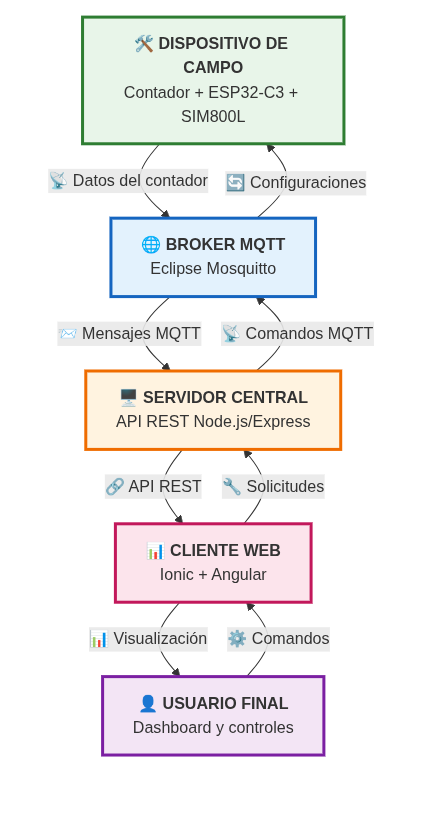
\includegraphics[width=0.4\linewidth]{./Figures/diagArq.png}
  \caption{Diagrama de arquitectura del sistema y el flujo de datos.}
  \label{fig:diag_arquitectura}
\end{figure}


\subsection{Decisiones de diseño clave}

\begin{itemize}

\item Separación broker/aplicación: permite cambiar broker o desplegar uno local sin tocar la lógica de negocio.

\item MQTT para mensajería ligera (QoS configurable) porque minimiza overhead en GPRS y facilita pub/sub.

\item API REST en Node.js/Express para exponer endpoints transaccionales y de gestión, centralizando autenticación y control de accesos.
\end{itemize}









